% !TEX root = ../memoria.tex

% Chapter 2

\chapter{Introducción específica}

En este capítulo se desglosan las diferentes herramientas, tanto de software como hardware, elegidas para el desarrollo del robot móvil propuesto en este trabajo.

\label{Chapter2}

\section{Robot Operating System}

ROS, el Sistema Operativo Robótico o \textit{Robot Operating System}, es un \textit{framework} de código abierto. ROS esta pensado para funcionar como una plataforma de software común para personas que diseñan y usan robots. La misma permite compartir código y y paquetes de una manera fácil y práctica lo cual permite minimizar el tiempo de desarrollo necesario para lograr que un robot comience a moverse.

\subsection{Descripción de la plataforma}

El ecosistema ROS esta compuesto de los siguientes elementos principales:

\begin{enumerate}
    \item Un set de drivers que permiten leer informacion desde sensores y comandar actuadores de manera abstraída del hardware y con un formato bien definido. Una gran variedad de hardware popular se encuentra actualmente soportada, incluyendo un enorme número de robots disponibles comercialmente.
    \item Una gran y creciente colección de algoritmos de robótica básicos o fundamentales para casi cualquier tipo de robot. Esto permite generar mapas del ``mundo'', navegarlo, representar e interpretar información generada por sensores, planear trayectorias, manipular objetos entre muhos otros. Gracias a la adopción de la plataforma en la comunidad acadpemica, una gran cantidad de algoritmos experimentales de última generación se encuentran disponibles para ROS.
    \item Una infrastructura computacional basada en grafos que permite ``mover'' información, interconectar los componentes de un sistema robótico complejo, además de incorporar piezas de software personalizadas, tales implementaciones de algoritmos propiios. ROS es inherentemente distribuido, lo que significa que es posible separar las cargas de trabajo de los distintos componentes que conforman el robot entre diferentes computadoras de manera totalmente transparente.
    \item Una gran cantidad de herramientas que facilitan la visualización del estado del robot y sus algoritmos, la depuración y el almacenamiento de datos recolectados o generados. La depuración del software de un robot es una tarea notablemente difícil, por lo que este set de herramientas constituye uno de los diferenciadores que hacen de ROS una plataforma tan potente como la es.
    \item Por último, el gran ecosistema de ROS incluye un set extensivo de recursos, tales como una wiki donde se documentan varios de los aspectos del framework, además de una plataforma de preguntas y respuestas muy activa entre los miembros de la comunidad.
\end{enumerate}

\subsection{Decisiones de diseño}

El diseño original de ROS se guió por las siguientes restricciones:

\begin{itemize}
    \item El \textit{stack} de la aplicación puede descomponerse en varios sub-sistemas independientes, como navegación, visión artificial, locomoción, etc.
    \item Los sub-sistemas pueden re-utilizarse en distintas tareas, tales como patrullas de seguridad, limpieza, sistemas de \textit{delivery}, etc.
    \item Mediante la correcta implementación de las capas abstracción de hardware y geometría del dispositivo, la mayor parte del software de aplicación puede reutilizarse en \textit{cualquier} robot.
\end{itemize}

En la siguiente sección se describen los principales componentes que hacen a un sistema ROS,

\subsection{El ROS Graph}

Estos requerimientos pueden ilustrarse mediante el sistema de representación fundamental de un sistema ROS: El ROS Graph. Un sistema ROS esta conformado por muchos programas distintos corriendo simultáneamente, los cuales se comunican entre sí mediante el paso de mensajes. Resulta conveniente el uso de un \textit{grafo} matemático para representar esta colección de programas y mensajes: los programas se representan mediante \textit{nodos} y los mismos se conectan entre sí mediante \textit{edges} o aristas. Típicamente, los nodos corresponden a procesos POSIX mientras que las aristas a conexiones TCP. Estas aristas representan el flujo de mensajes entre dos nodos, tal como puede apreciarse en la figura \ref{fig:rosNodeGraph}.

\begin{figure}[ht]
    \centering
    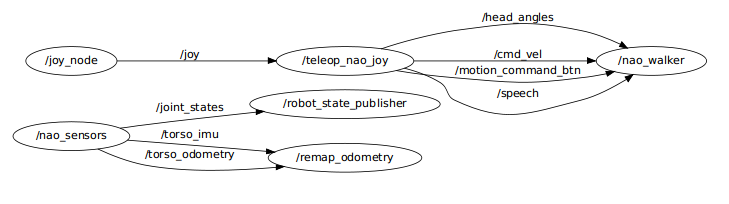
\includegraphics[scale=.6]{./Figures/ros_node_graph.png}
    \caption{Ejemplo de un ROS Node Graph. Los nodos en el grafo representan los programas individuales. Las aristas representan el flujo de información entre los diferentes nodos.}
    \label{fig:rosNodeGraph}
\end{figure}

Entre otras ventajas, esta arquitectura ofrece un nivel de tolerancia a fallos adicional: un crash en una de las piezas de software típicamente solo echará abajo a su proceso asociado, mientras que el resto del grafo seguirá funcionando de manera normal. Las circunstancias del fallo podrán luego ser recreadas de manera sencilla grabando los mensajes que entran y salen de ese nodo en particular en un log y luego reproduciéndolo como si se tratase de una pista de sonido.

Hasta este punto se ha asumido que los nodos son capaces de encontrarse unos con otros pero todavía no se ha expuesto como funciona este sistema. La respuesta esta en un programa llamado \texttt{roscore}.

\subsubsection{Roscore}

El roscore es un servicio que provee de la información necesaria a los nodos, de modo a que estos puedan transmitir mensajes unos a otros. Cada nodo se conecta individualmente al roscore al momento de iniciarse para registrar los detalles sobre los mensajes que este publica y los que desea recibir. Cuando un nuevo nodo aparece, el roscore lo abastece con la información que este necesita para conformar una comunicación directa o \textit{peer-to-peer} con otros nodos publicando y suscribiéndose al mismo tópico de mensaje. Cada sistema ROS necesita de un roscore corriendo ya que sin el, los nodos no serían capaces de encontrarse entre sí, aún así, la interacción real entre el roscore y el nodo se realiza solo al momento en que el nodo es lanzado, tal como se demuestra en la figura \ref{fig:roscoreAndNodes}.

\begin{figure}[ht]
    \centering
    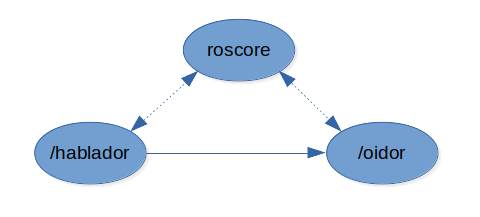
\includegraphics[scale=.6]{./Figures/diagrama_nodos.png}
    \caption{El roscore se conecta solo de manera efímera con otros nodos en el sistema.}
    \label{fig:roscoreAndNodes}
\end{figure}

\subsubsection{Tópicos}

Como ya se vió en el apartado anterior, un sistema ROS consiste en un número de nodos independientes que se relacionan en un grafo. Un nodo por si solo no resulta especialmente útil, pero el conjunto se vuelve realmente potente una vez que los pares empiezan a comunicarse unos con otros e intercambiar información. El canal más típico para este intercambio de mensajes se lleva a cabo a través de tópicos, una de las interpretaciones de las aristas de un grafo. Un tópico es el nombre dado a un canal de comunicaciones capaz de pasar mensajes de un tipo definido. Por ejemplo, la información de un escáner láser 2D podría transmitirse en un tópico llamado \texttt{/scan}, con un mensaje del tipo \texttt{LaserScan}, mientras que la información de una cámara modría enviarse a través de un tópico llamado \texttt{/image}, con un mensaje del tipo \texttt{Image}.


\subsection{Espacios de trabajo o workspaces}

Un \textit{workspace} ROS es simplemente un conjunto de directorios dentro de los cuales reside un conjunto de código ROS. En general, un workspace representa un conjunto de paquetes que implementan funcionalidades distintas y que son integrados juntos para una finalidad particular. Es posible tener múltiples workspaces ROS, pero solo es posible trabajar en uno de ellos a la vez, ya que para un paquete solo es posible ``ver'' código que reside dentro del mismo workspace que él. Por ejemplo, para el desarrollo de este trabajo final se hizo uso de un solo workspace. La estructura típica de un workspace ROS podría verse así:

\begin{lstlisting}[basicstyle=\ttfamily, keywords={}]
cese_ws/
`-- src
    `-- cese-bot
        |-- CMakeLists.txt
        |-- package.xml
        |-- include
        |   `-- robot_node.h
        `-- src
            `-- robot_node.cpp
\end{lstlisting}




\subsection{Paquetes}

El software desarrollado utilizando ROS se encuentra organizado en paquetes o \textit{rospackages}, cada uno de los cuales contiene alguna combinación de código y documentación. Estos paquetes funcionan de manera similar a los paquetes que pueden instalarse en Ubuntu vía el comando \texttt{apt}. El ecosistema ROS contiene miles de paquetes disponibles en repositorios abiertos, los cuales pueden ser fácilmente instalados para ser aprovechado por cualquier usuario.

Los paquetes se ubican dentro del directorio \texttt{src}. Cada uno de estos paquetes debe incluir un archivo \textit{CMakeLists.txt} y un \textit{packages.xml} que describe el contenido de los mismos así como indicar a catkin cómo interactuar con los mismos.

\subsection{Sistema de compilación catkin}

\texttt{catkin} es el sistema de compilación defacto de ROS. Este consiste en un set de herramientas que ROS utiliza para generar ejecutables, librerías, scripts e interfaces que pueden ser utilizadas por otras plataformas. Catkin resulta indispensable para trabajar en lenguaje C++ con ROS.
Catkin esta formado por un conjunto de macros de \texttt{CMake} y scripts de Python que proveen funcionalidad añadida al CMake tradicional de modo a facilitar su uso por parte del roboticista.

\subsection{RViz}

RViz son las siglas de ROS Visualization. Es un entorno de visualización en 3D de propósito general para robots, sensores y algoritmos. Como la mayoría de las herramientas de ROS, puede ser usado para cualquier robot y rápidamente adaptado a una aplicación en particular. RViz es capaz de mostrar una variedad de tipos de dato transmitidos a través de un sistema ROS con énfasis especial, pero no limitado a, tipos de datos representables en tres dimensiones.

Así como otros sistemas complejos con interfaz gráfica, RViz posee un número de paneles y plugins que pueden ser configurados según necesidad para una tarea en particular, como el mostrado en la figura \ref{fig:rvizScreenshot}. Configurar RViz correctamente puede tomar cierto tiempo, por lo que es posible guardar la configuración del mismo en un archivo para usarse en la posteridad. En este trabajo se incluyen dos de estos archivos de configuración, uno para la generación del mapa y otro para la navegación del robot.

% TODO: agregar referencias a los archivos en github

\begin{figure}[ht]
    \centering
    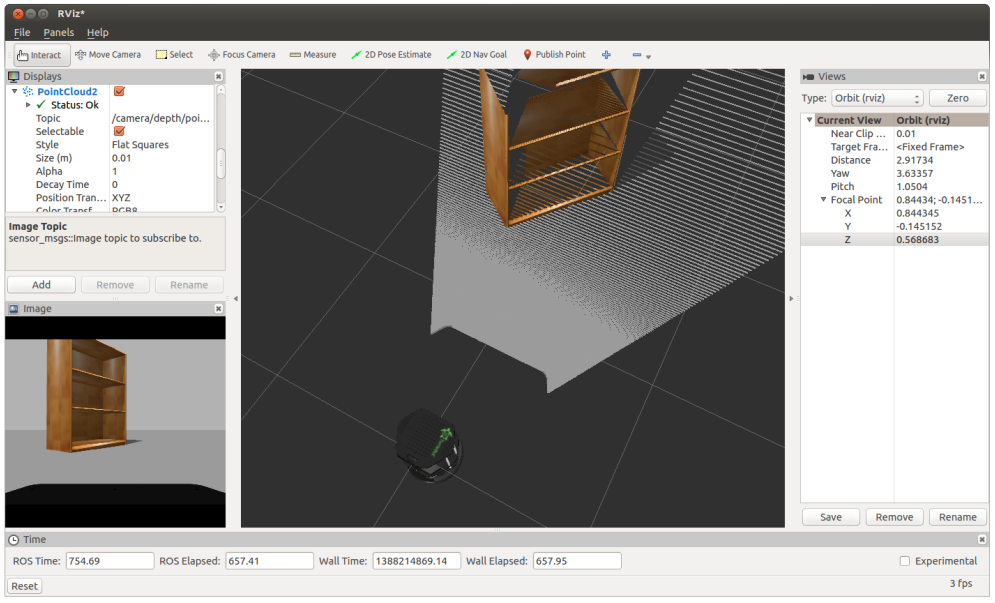
\includegraphics[scale=.3]{./Figures/rviz_screenshot.png}
    \caption{El panel de RViz cargado con un panel adicional para visualización de cámara durante una simulación.}
    \label{fig:rvizScreenshot}
\end{figure}

%----------------------------------------------------------------------------------------
%	SECTION 2
%----------------------------------------------------------------------------------------

\section{iRobot Roomba 500/600}

La serie Roomba es una gama de robots domésticos de limpieza, producidos por la empresa estadounidense iRobot. Estos robots se caracterizan por disponer de un puerto serie como el que se aprecia en la figura \ref{fig:roombaSerialPort}, destinado originalmente a procesos de depuración, mediante el cual es posible comunicarse bi-direccionalmente con el robot permitiendo, entre otras cosas, la lectura de sus sensores y el comando de sus actuadores. Esta comunicación se realiza mediante un protocolo propio de la empresa denominado Open Interface\protect\footnotemark que ha sido liberado al público para utilizarse en proyectos de \textit{STEM}, por sus siglas en inglés: ciencia, tecnología, ingeniería y matemáticas.

\footnotetext{\url{https://www.irobot.lv/uploaded_files/File/iRobot_Roomba_500_Open_Interface_Spec.pdf}}


\begin{figure}[ht]
    \centering
    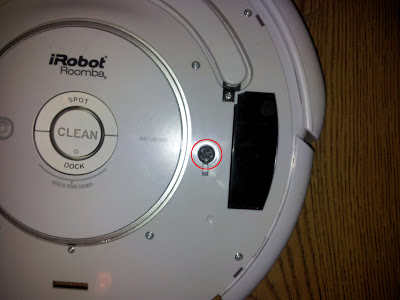
\includegraphics[scale=.5]{./Figures/roomba_serial_port.jpg}
    \caption{Puerto serie de depuración en robot Roomba 550.}
    \label{fig:roombaSerialPort}
\end{figure}

Existe una variedad importante de robots Roomba, principalmente gracias a que la plataforma posee ya 17 años en el mercado. Por este motivo, resulta importante describir los modelos compatibles con este trabajo: todos los modelos de la serie 500 y 600. Estos, además de incluir el puerto de la Open Interface, disponen de sensores de mayor definición y precisión que la serie 400. Las series posteriores como la 700 en adelante, ya no disponen del puerto Open Interface por lo que debieron quedar descartadas.


%-----------------------------------
%	SUBSECTION 2.1
%-----------------------------------

\subsection{Protocolo Open Interface}

El protocolo Roomba Open Interface (OI), es una interfaz para controlar y manipular el comportamiento del robot Roomba. Esta interface permite manipular el comportamiento del robot, así como leer el estado de sus sensores a través de comandos serie que uno envía al robot conectando el puerto a una PC o microcontrolador mediante un conector Mini-DIN.


\subsection{Conexión física}

Para utilizar el OI; un procesador capaz de manipular un puerto serie, tal como una PC o microcontrolador, debe conectarse al conector externo Mini-DIN del que dispone la Roomba. Este conector ofrece una comunicación serie bi-direccional con niveles de tensión TTL (0 - 5 VCC). El mismo provee además de un pin de tensión no-regulada, conectada directamente a la batería de la Roomba. Para acceder a este puerto es necesario remover primeramente la careta plástica de la parte superior del robot.

\subsubsection{Distribución de pines del conector Mini-DIN}

En la figura \ref{fig:roscoreAndNodes} se muestra la distribucion de pines del conector hembra de la Roomba y en la tabla \ref{fig:cuadradoAzul} se describen cada uno de los mismos.


\begin{figure}[ht]
    \centering
    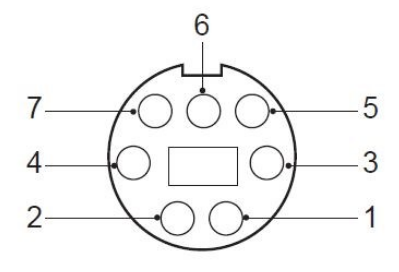
\includegraphics[scale=.4]{./Figures/pinout.png}
    \caption{Distribución de pines en el conector hembra Mini-DIN.}
    \label{fig:roombaPinout}
\end{figure}


\begin{table}[h]
    \centering
    \caption{Referencia de pines en conector Mini-DIN hembra}
    \label{tab:Pines}
    \begin{tabular}{rll}
        \toprule
        \multicolumn{1}{l}{Pin} & Nombre & Descripción                        \\
        \midrule
        1                       & Vpwr   & Directo de batería + (no regulado) \\
        2                       & Vpwr   & Directo de batería + (no regulado) \\
        3                       & RXD    & 0 - 5 VCC Entrada serie            \\
        4                       & TXD    & 0 - 5 VCC Salida serie             \\
        5                       & BRC    & Cambio de baud-rate                \\
        6                       & GND    & Tierra del robot                   \\
        7                       & GND    & Tierra del robot                   \\
        \bottomrule
    \end{tabular}
\end{table}
%----------------------------------------------------------------------------------------
%	SECTION 3
%----------------------------------------------------------------------------------------
\section{Placa de desarollo NUCLEO-F746ZG}

La placa NUCLEO-F746ZG es un producto ofrecido por el fabricante ST como una plataforma de prototipado rápido basado en el microcontrolador STM32F746ZG. La misma se caracteriza por contar con un controlador Ethernet integrado, un programador-debugger que además puede funcionar como interfaz RS-232/USB, especialmente útil para tareas de desarrollo y depuración.

Este microcontrolador dispone de un núcleo ARM Cortex-M7 que corre a frecuencias de hasta 216 MHz. Posee además, 1 Mbyte de memoria tipo flash, y 320 KB de memoria RAM. Destaca por su gran cantidad de periféricos, los cuales son fácilmente configurables a través de la plataforma STM32CubeMX, una interfaz gráfica de configuración para microcontroladores ST que permite, además de inicializar periféricos, integrar middlewares de terceros tales como FreeRTOS, LwIP, etc., con una simplicidad sin precedentes. En la figura \ref{fig:stm32CubeMX} se puede apreciar una de las pantallas de configuración de la aplicación.

\begin{figure}[ht]
    \centering
    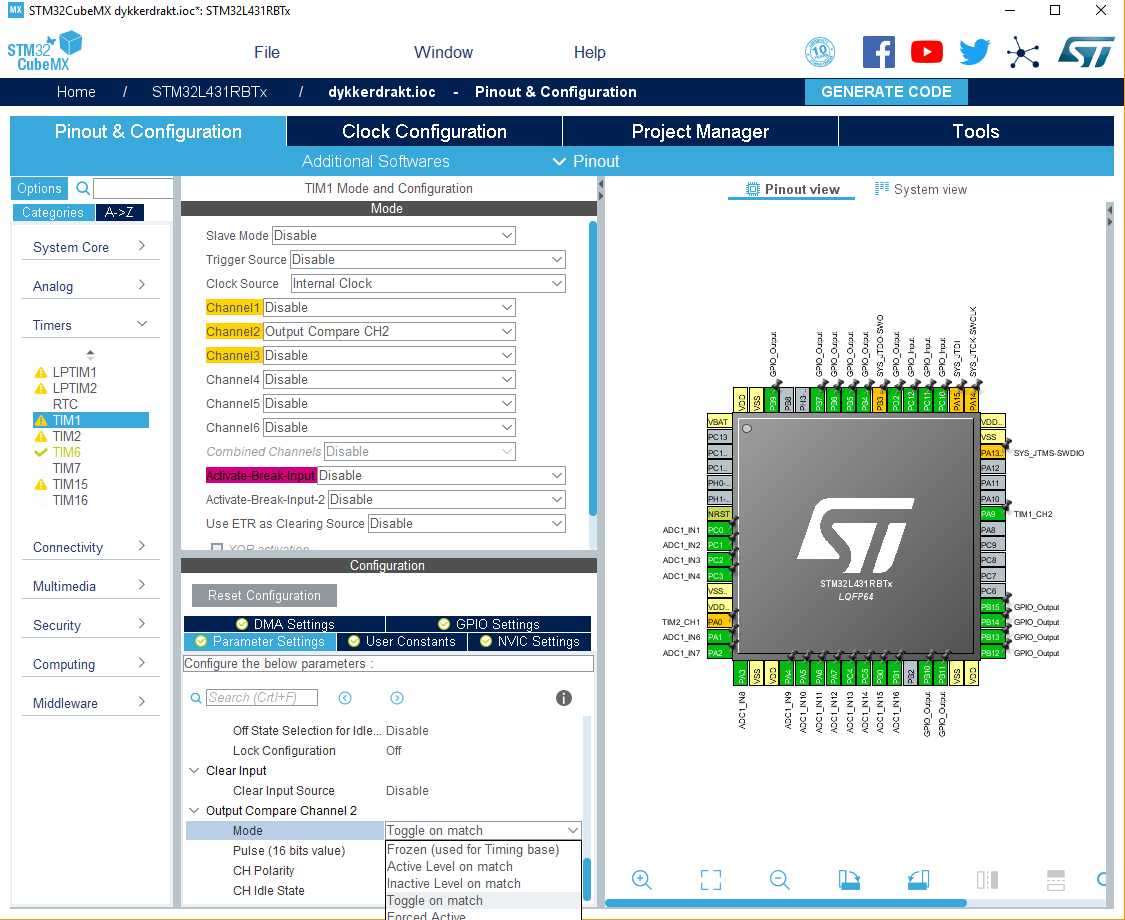
\includegraphics[scale=.3]{./Figures/stm32_cubemx.png}
    \caption{Configuración de un microcontrolador a través de la aplicación STM32CubeMX.}
    \label{fig:stm32CubeMX}
\end{figure}

Resulta importante destacar que esta aplicación permite la exportación de proyectos pre-generados hacia una amplia variedad de IDEs comerciales y gratuitos, además de una opción basada en Makefiles, especialmente útil para su uso en flujos de trabajo más ``minimalistas'', como los basados en editores de texto avanzados y línea de comandos.



% M7, Ethernet, RAM


%----------------------------------------------------------------------------------------
%	SECTION 5
%----------------------------------------------------------------------------------------
\section{Computadora OrangePI PC}

La OrangePI PC es una \textit{Single Board Computer} de hardware abierto, es decir que tanto sus esquemáticos como el firmware de la misma se encuentran disponibles de manera pública. Este dispositivo es, en factor de forma y características, similar a la ampliamente conocida Raspberry PI, pero con un precio de venta aún mas moderado, lo que la vuelve una alternativa interesante para este trabajo, en que se busca reducir costos.

Esta placa disponde de un microprocesador Allwinner de 32bit y 4 núcleos, y cuenta con 1 GB de memoria RAM DDR3. Es compatible con una amplia gama de sistemas operativos y distribuciones, y para este trabajo en particular, se decidió utilizarla con Ubuntu 14.04. Esta decisión viene ligada a que ROS Indigo, la versión de ROS compatible con este sistema, es la más ampliamente difundida y la que dispone de una mayor cantidad de paquetes.

\begin{figure}[ht]
    \centering
    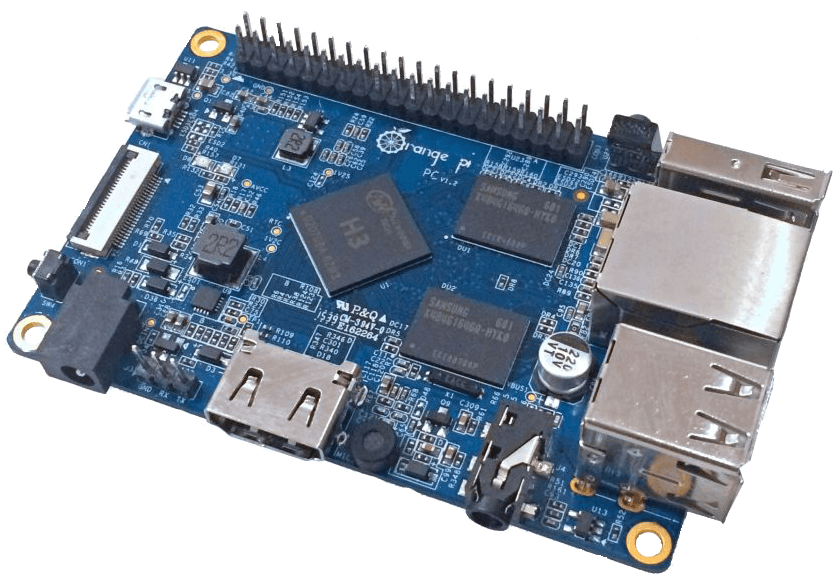
\includegraphics[scale=.2]{./Figures/orangepi.png}
    \caption{Vista superior de la SBC OrangePI PC, alternativa económica al Raspberry PI.}
    \label{fig:orangePI}
\end{figure}

En la figura \ref{fig:orangePI} se muestra una vista superior de la placa OrangePI PC donde se pueden apreciar sus conectores y layout, muy similares a los de la Raspberry PI 2. Para este trabajo, se hizo uso del conector ethernet así como de 2 de sus 3 puertos USB 2.0.


%----------------------------------------------------------------------------------------
%	SECTION 6
%----------------------------------------------------------------------------------------
\section{Sensor Kinect para Xbox 360}

El Kinect para Xbox 360 o simplemente Kinect, es un dispositivo de captura de movimiento diseñado por la empresa Microsoft, utilizando la tecnología desarrollada por la empresa israelita PrimeSense. El dispositivo cuenta con una cámara RGB, un sensor de profundidad, un micrófono de múltiples matrices y un procesador personalizado, que proporcionan, al utilizarse en una consola Xbox 360, captura de movimiento de todo el cuerpo en 3D, reconocimiento facial y capacidades de reconocimiento de voz.

El sensor de profundidad es un proyector de infrarrojos combinado con un sensor CMOS monocromo que permite al Kinect generar un \textit{Depth Map}
o mapa de profundidad, es decir, una imagen que contiene información relativa a la distancia de las superficies presentes en una escena con respecto a un punto de vista determinado. En la figura \ref{fig:depthImage} se puede apreciar el Depth Map generado por el sensor Kinect en el que se puede distinguir la silueta de una persona en una habitación. Las tonalidades de grises son una representación de la distancia por lo que para puntos cercanos veremos un pixel mas claro, mientras que para puntos mas lejanos veremos píxeles mas oscuros.

\begin{figure}[ht]
    \centering
    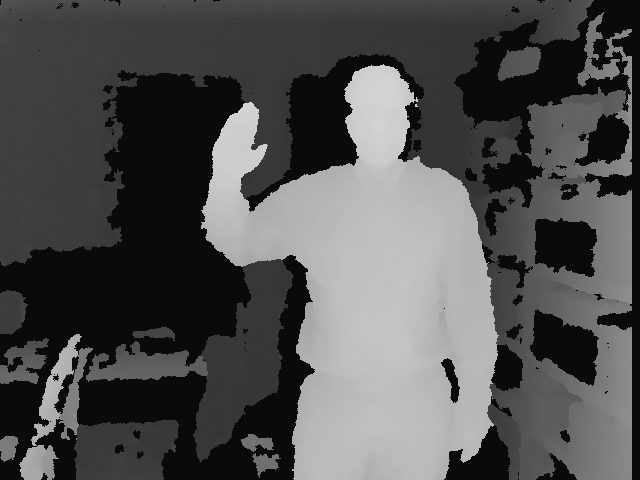
\includegraphics[scale=.3]{./Figures/depth_image.png}
    \caption{Ejemplo de un Depth Map generado por el sensor Kinect.}
    \label{fig:depthImage}
\end{figure}

Gracias al desarrollo de un conjunto de controladores open source llamado freenect\protect\footnotemark, el uso del sensor Kinect se ha extendido a sistemas operativos del tipo GNU/Linux y con esto, su introdución al universo ROS. Al día de hoy, exisen una serie de paquetes listos para usar que permiten consumir la información de profundidad, cámara RGB y micrófonos directamente desde tópicos ROS.


\subsection{Limitaciones}

Como ya se mencionó anteriormente, el sensor de profundidad del Kinect funciona gracias a un proyector de puntos de luz en el espectro infrarrojo y en una cámara especializada diseñada para captar los haces rebotantes.

Un detalle importante a tener en cuenta a la hora de decidir si el Kinect es el sensor adecuado para una aplicación en particular es la incapacidad de éste de funcionar en entornos con luz solar directa. Esto viene dado a que la luz solar abarca el espectro electromagnético comprendido entre longitudes de onda 250 hasta 2500 nanometros donde es incluye pequeño el espectro de luz infrarroja utilizado por el sensor Kinect. Esto genera lecturas erroneas que hacen al sensor totalmente inutilizable bajo dichas circunstancias.

% Salvando distancias entre una cámara de profundidad y un sensor LIDAR, en determinados escenarios es posible remplazar un costoso sensor LIDAR con un Kinect, procesando el mapa de puntos en 3D y generando un LaserScan en 2D a partir de uno de los múltiples planos que lo componen. Esta información ya procesada, puede utilizarse para alimentar paquetes de ROS diseñados para consumir datos generados por un LIDAR.
% \footnotetext{\url{https://github.com/OpenKinect/libfreenec}}

% Descripción, disponibilidad y restricciones de uso.
% Imagen de un pointcloud raw
